% !TEX root = ../ApproxDA-TransUNet.tex
\section{Global Context Sensitivity and the Semantic Spatial Dependency Mechanism}
\label{sec:gcs_mechanism}
\label{sec:understanding}

Section~\ref{sec:experiments} demonstrated that the impact of attention approximation is deeply task-dependent. This section investigates the theoretical and empirical underpinnings of this phenomenon. We establish the empirical spectrum of Global Context Sensitivity (GCS), systematically eliminate alternative geometric and modality-based explanations through causal analysis, and identify Semantic Spatial Dependency (SSD) as the unifying mechanism governing attention approximation in medical segmentation.

\subsection{Empirical Window Sensitivity and the GCS Spectrum}
\label{sec:approx_scale}
\label{sec:obs2}

We first examine how spatial approximation scale (window size $M$) impacts segmentation accuracy across different biomedical imaging tasks. Table~\ref{tab:window_ablation} isolates this effect on Synapse multi-organ CT by varying $M \in \{7, 14, 28, 56, 112\}$ under fixed gate=pam, $r{=}32$.

\begin{table}[ht]
  \caption{Spatial Approximation Ablation on Synapse ($G$=8)}
  \label{tab:window_ablation}
  \centering
  \setlength{\tabcolsep}{2pt}
  \small
  \begin{tabular}{lccccc}
    \toprule
    Config & $M$ & $r$ & Gate & DSC (\%) $\uparrow$ & HD95 (mm) $\downarrow$ \\
    \midrule
    Windowed + low-rank & 7   & 32 & pam          & 78.64          & 31.09 \\
    Windowed + low-rank & 14  & 64 & learn$^\dag$ & 78.04          & 29.09 \\
    Windowed + low-rank & 28  & 32 & pam          & \textbf{80.94} & \underline{27.49} \\
    Windowed + low-rank & 56  & 32 & pam          & 78.90          & 35.23 \\
    Global + low-rank   & 112 & 32 & pam          & \underline{79.44} & \textbf{27.26} \\
    \bottomrule
  \end{tabular}
  \par\vspace{5pt}
  \parbox{\columnwidth}{\footnotesize $^\dag$Gate collapsed to $g{\approx}0.5$. $M{=}112$ via window clamping yields full-map attention at all scales.}
\end{table}

The Synapse DSC-vs-$M$ curve exhibits a clear non-monotonic profile: performance peaks at $M{=}28$ (80.94\% DSC, $+$1.14\% over DA-TransUNet), while overly local ($M{=}7$: 78.64\%) and overly global ($M{=}112$: 79.44\%) scopes underperform. This behavior mirrors a bias-variance tradeoff: insufficient receptive fields miss critical cross-organ context, whereas unrestricted global attention admits non-informative long-range correlations from irrelevant background tissue.

\begin{figure}[!t]
\centering
\scalebox{1.0}{%
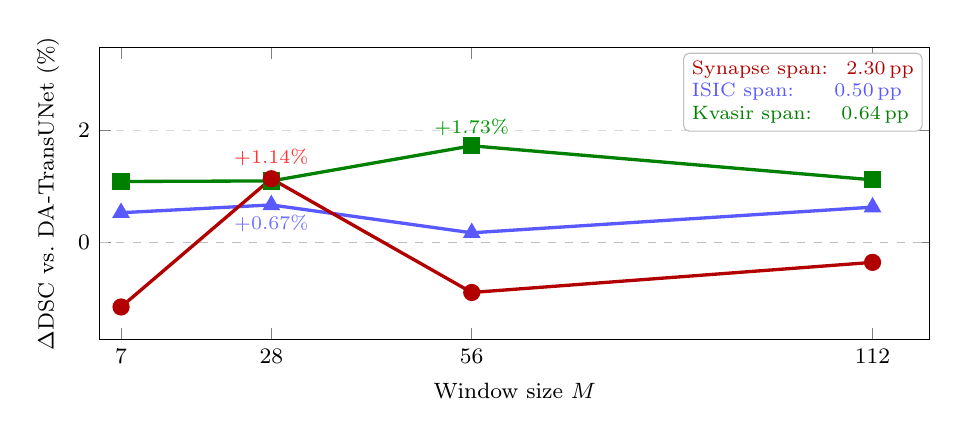
\begin{tikzpicture}
\begin{axis}[
  width=\columnwidth, height=5.3cm,
  xlabel={Window size $M$},
  ylabel={$\Delta$DSC vs.\ DA-TransUNet (\%)},
  ymin=-1.75, ymax=3.5,
  xtick={7,28,56,112},
  xticklabels={7,28,56,112},
  xmin=4, xmax=120,
  ymajorgrids=true,
  grid style={dashed,gray!30},
  tick label style={font=\footnotesize},
  label style={font=\footnotesize},
  every axis plot/.append style={very thick, mark size=2.5pt},
]
% Zero reference
\addplot[dashed, gray!50, very thin, forget plot] coordinates {(4,0)(120,0)};
% ISIC 2018 (drawn first, behind)
\addplot[color=blue!65, mark=triangle*]
  coordinates {(7,0.53) (28,0.67) (56,0.17) (112,0.63)};
% Kvasir-SEG (drawn second)
\addplot[color=green!50!black, mark=square*]
  coordinates {(7,1.09) (28,1.10) (56,1.73) (112,1.12)};
% Synapse (drawn last — on top of all other lines)
\addplot[color=red!70!black, mark=*]
  coordinates {(7,-1.16) (28,1.14) (56,-0.90) (112,-0.36)};
% Peak label — Synapse
\node[font=\scriptsize, color=red!80, anchor=south]
  at (axis cs:28,1.2) {$+$1.14\%};
% Peak label — ISIC (below point to avoid curves above)
\node[font=\scriptsize, color=blue!55, anchor=north]
  at (axis cs:28,0.67) {$+$0.67\%};
% Peak label — Kvasir
\node[font=\scriptsize, color=green!60!black, anchor=south]
  at (axis cs:56,1.73) {$+$1.73\%};
% Span annotation box
\node[anchor=north east, align=left, font=\scriptsize,
      fill=white, draw=gray!50, inner sep=3pt, rounded corners=2pt]
  at (axis cs:119, 3.40) {%
    \textcolor{red!70!black}{Synapse span:\phantom{0} 2.30\,pp}\\
    \textcolor{blue!65}{ISIC span:\phantom{000} 0.50\,pp}\\
    \textcolor{green!50!black}{Kvasir span:\phantom{00} 0.64\,pp}};
\end{axis}
\end{tikzpicture}}
\caption{$\Delta$DSC vs.\ window size $M$ (gate=pam, $r{=}32$) across representative tasks spanning the GCS spectrum. Curve colors: Synapse (red), ISIC~2018 (blue), Kvasir-SEG (green).}
\label{fig:dsc_vs_m}
\end{figure}

To quantify task sensitivity across benchmarks, we define empirical \textbf{Global Context Sensitivity (GCS)} as the maximum performance span across window scales:
\begin{equation}
  \Delta\text{DSC} = \max_{M} \text{DSC}(M) - \min_{M} \text{DSC}(M),
  \label{eq:gcs}
\end{equation}
measured under gate=pam, $r{=}32$. As summarized in Table~\ref{tab:gcs_spectrum} and Figure~\ref{fig:dsc_vs_m}, tasks form a structured spectrum spanning a $4.6\times$ sensitivity difference:
\begin{itemize}
  \item \textbf{High-GCS Tier (Synapse, $\Delta\text{DSC} = 2.30$\,pp):} Steep performance curve with a sharp optimum at $M{=}28$. Window choice is critical to accuracy.
  \item \textbf{Low-GCS Tier (ACDC, Kvasir, CVC, ISIC, $\Delta\text{DSC} \le 0.73$\,pp):} Broad performance plateaus where any local window ($M \in \{7, 28, 56\}$) achieves competitive or superior performance relative to global attention.
\end{itemize}

\begin{table}[tb]
  \caption{Empirical GCS Spectrum ($\Delta$DSC) Across Five Biomedical Segmentation Benchmarks (gate=pam, $r{=}32$).}
  \label{tab:gcs_spectrum}
  \centering
  \setlength{\tabcolsep}{6pt}
  \begin{tabular}{llcc}
    \toprule
    Dataset & Modality / Anatomy & Classes & $\Delta$DSC (pp) \\
    \midrule
    Synapse      & Multi-organ CT      & 9 & \textbf{2.30} (High GCS) \\
    ACDC         & Cardiac MRI         & 4 & 0.73 (Low GCS) \\
    Kvasir-SEG   & Polyp (endoscopy)   & 2 & 0.64 (Low GCS) \\
    CVC-ClinicDB & Polyp (colonoscopy) & 2 & 0.62 (Low GCS) \\
    ISIC 2018    & Skin lesion         & 2 & 0.50 (Low GCS) \\
    \bottomrule
  \end{tabular}
\end{table}

\subsection{Causal Elimination of Competing Hypotheses}
\label{sec:causal_elimination}

What intrinsic property of a medical segmentation task drives its GCS tier? We conduct a systematic causal elimination study using training-free annotation mask statistics computed across 200 randomly sampled masks per dataset. We formulate and test five candidate explanatory hypotheses:
\begin{itemize}
  \item \textbf{SC1 --- Foreground Area Ratio:} Fraction of foreground pixels. Tests if target scale dictates window sensitivity.
  \item \textbf{SC2 --- Boundary Complexity:} Mean isoperimetric ratio ($P^2/4\pi A$) per component. Tests if boundary irregularity drives GCS.
  \item \textbf{SC3 --- Spatial Entropy:} Normalized foreground entropy over an $8{\times}8$ grid. Tests if target dispersion determines context requirements.
  \item \textbf{SC4 --- Window Crossing Ratio (WCR):} Fraction of foreground pixels belonging to connected components spanning more than one $M{\times}M$ window ($M{=}28$~px in pixel space). Tests if component-level window boundary crossing drives sensitivity.
  \item \textbf{SC5 --- Inter-Class Window Separation:} Fraction of semantic class-centroid pairs falling in distinct $M{\times}M$ windows (structural zero for binary datasets). Measures whether multi-class reasoning requires cross-window communication.
\end{itemize}

A valid causal factor must achieve strong positive rank correlation ($\rho > 0.8$) with the empirical GCS ranking across all five datasets (Synapse $>$ ACDC $>$ Kvasir $\approx$ CVC $>$ ISIC). Table~\ref{tab:causal} and Figures~\ref{fig:causal}--\ref{fig:proxy} present the elimination results.

\begin{table*}[tb]
  \caption{Empirical verification of causal hypotheses ($M{=}28$, five benchmarks).}
  \label{tab:causal}
  \centering
  \small
  \setlength{\tabcolsep}{5pt}
  \begin{tabular}{llcccccccl}
    \toprule
    Hypothesis & Metric & Synapse & ACDC & Kvasir & ISIC & CVC & Spearman $\rho$ & Outcome \\
    \midrule
    SC1 & Foreground ratio       & 0.077  & 0.040 & 0.152 & 0.214 & 0.094 & $-$0.80 & \textbf{Ruled out} (Negative trend) \\
    SC2 & Boundary complexity    & 1.355  & 0.928 & 1.023 & 1.261 & 1.163 & $+$0.00$^\dagger$ & \textbf{Ruled out} (Zero correlation) \\
    SC3 & Spatial entropy        & 0.497  & 0.359 & 0.566 & 0.605 & 0.482 & $-$0.50 & \textbf{Ruled out} (Negative trend) \\
    SC4 & WCR ($M{=}28$~px)   & 0.999  & 0.954 & 1.000 & 0.999 & 1.000 & $-$0.37 & \textbf{Ruled out} (Saturates / Neg.) \\
    SC5 & Inter-class separation & \textbf{0.9996} & \textbf{0.547} & 0.000 & 0.000 & 0.000 & \textbf{+0.89} & \textbf{Strongest Predictor} \\
    \midrule
    Proxy & Class count ($n_\text{classes}$) & 3.99 & ${\approx}3.00$ & 1.00 & 1.00 & 1.00 & $+$0.87$^\ddagger$ & \textbf{Falsified by ACDC} (Proxy only) \\
    \bottomrule
  \end{tabular}
  \par\vspace{5pt}
  \parbox{\textwidth}{\footnotesize $^\dagger$Spurious partial correlation on 3 datasets ($\rho{=}+0.50$) collapsed to $\rho{=}0.00$ with 5 datasets.
  $^\ddagger$$n_\text{classes}$ is falsified as a true cause because ACDC has multi-class anatomy yet low GCS.}
\end{table*}

\begin{figure*}[tbp]
  \centering
  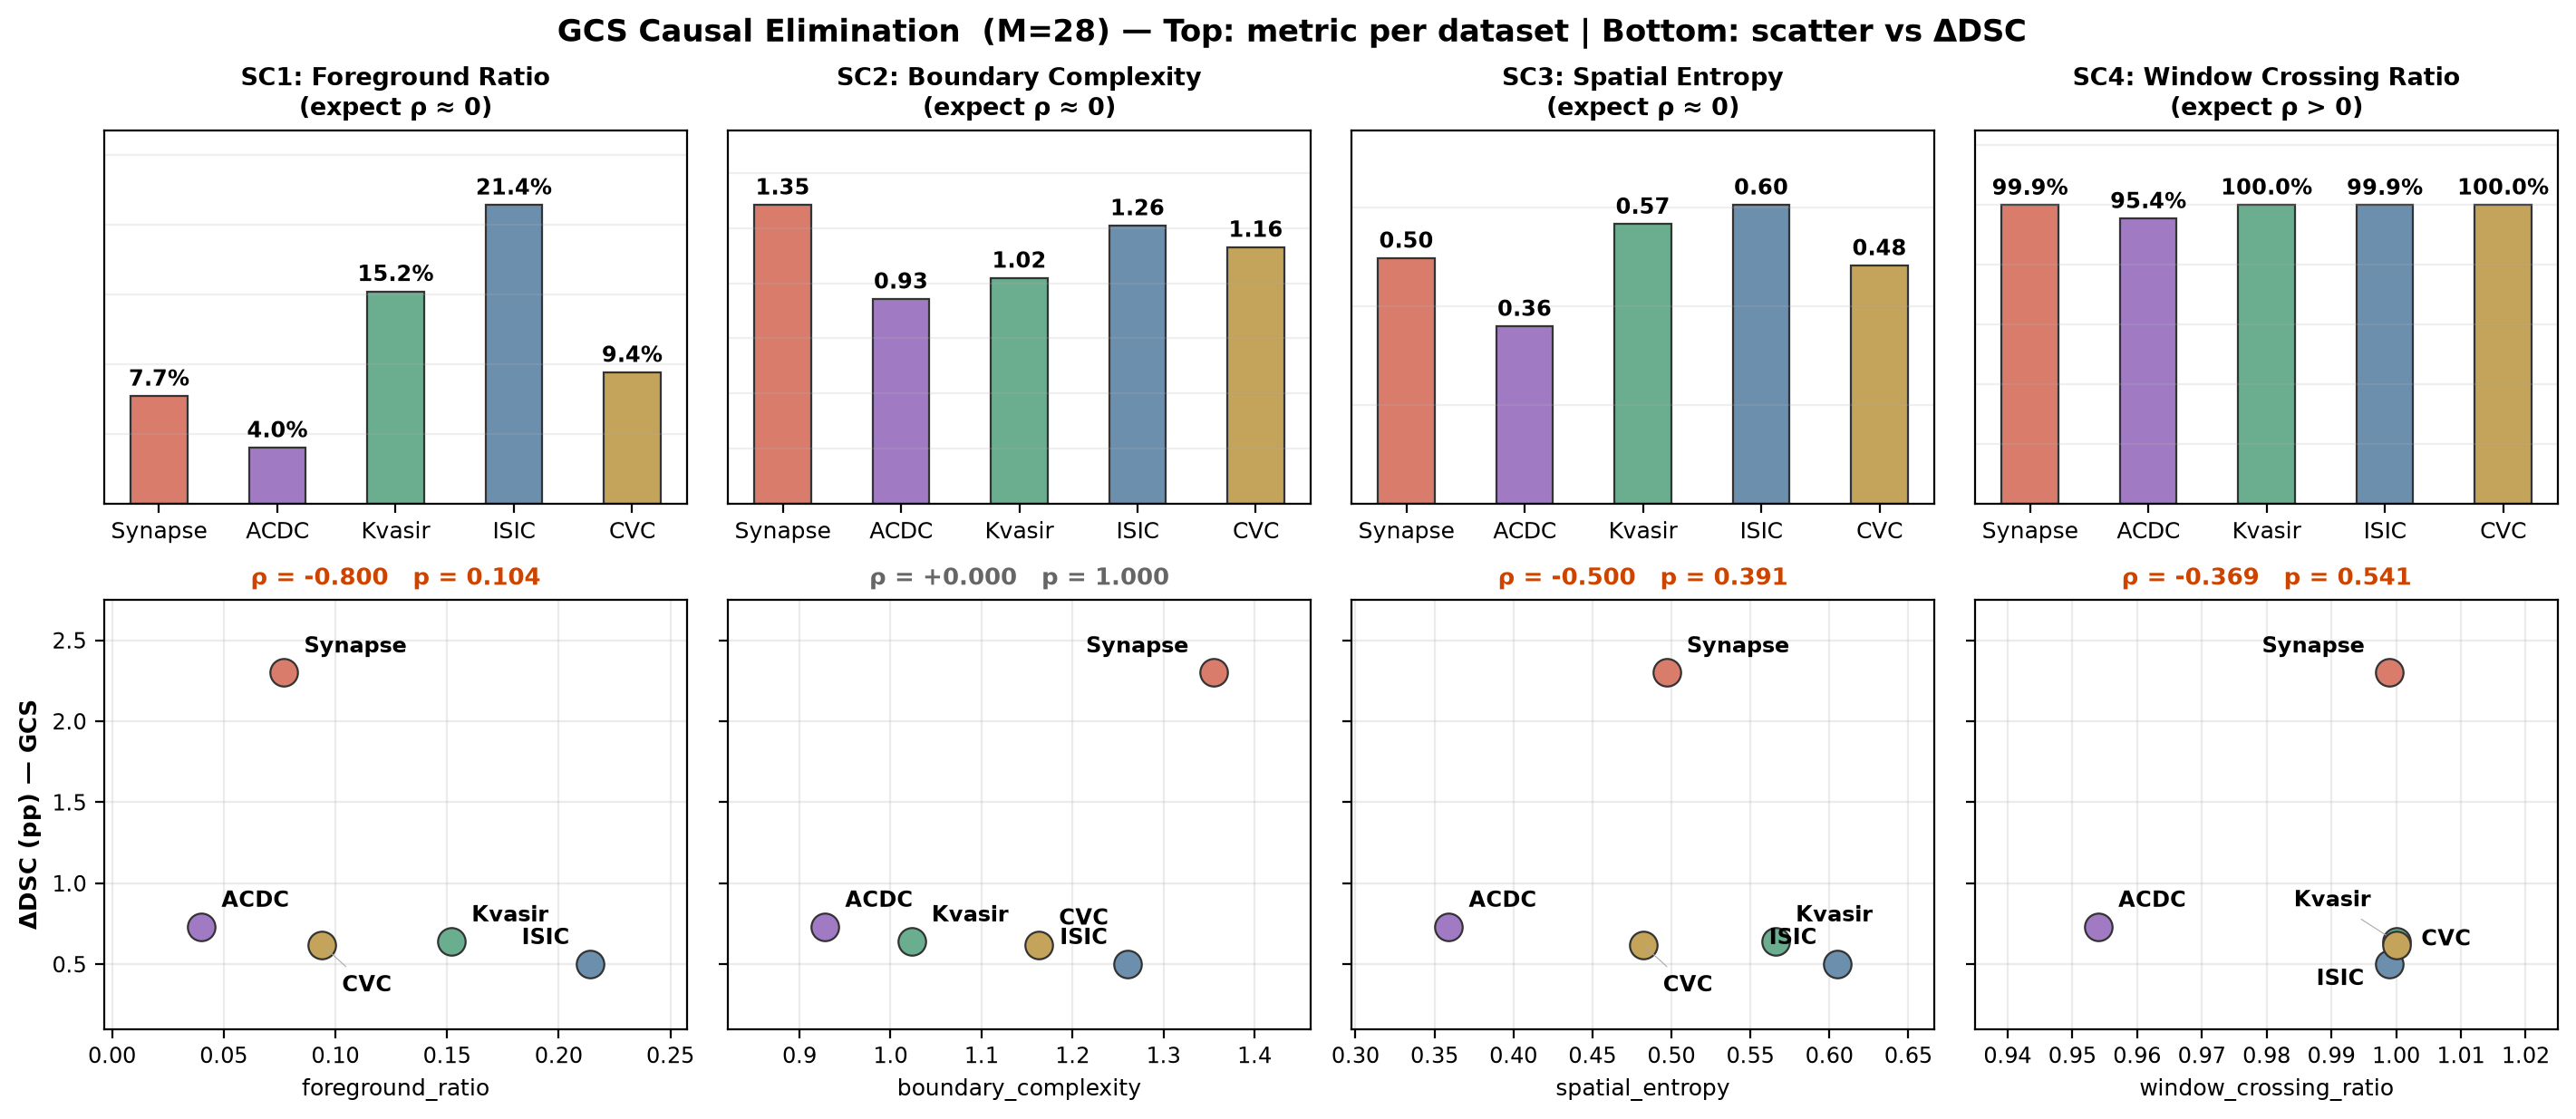
\includegraphics[width=\textwidth]{figures/gcs_causal_sanity.png}
  \caption{Causal elimination results across five benchmarks ($M{=}28$). Top row: per-dataset metric distributions. Bottom row: metric values vs.\ empirical $\Delta$DSC (GCS). SC5 (inter-class window separation, $\rho{=}+0.89$) stands as the sole surviving predictor.}
  \label{fig:causal}
\end{figure*}

\begin{figure*}[tbp]
  \centering
  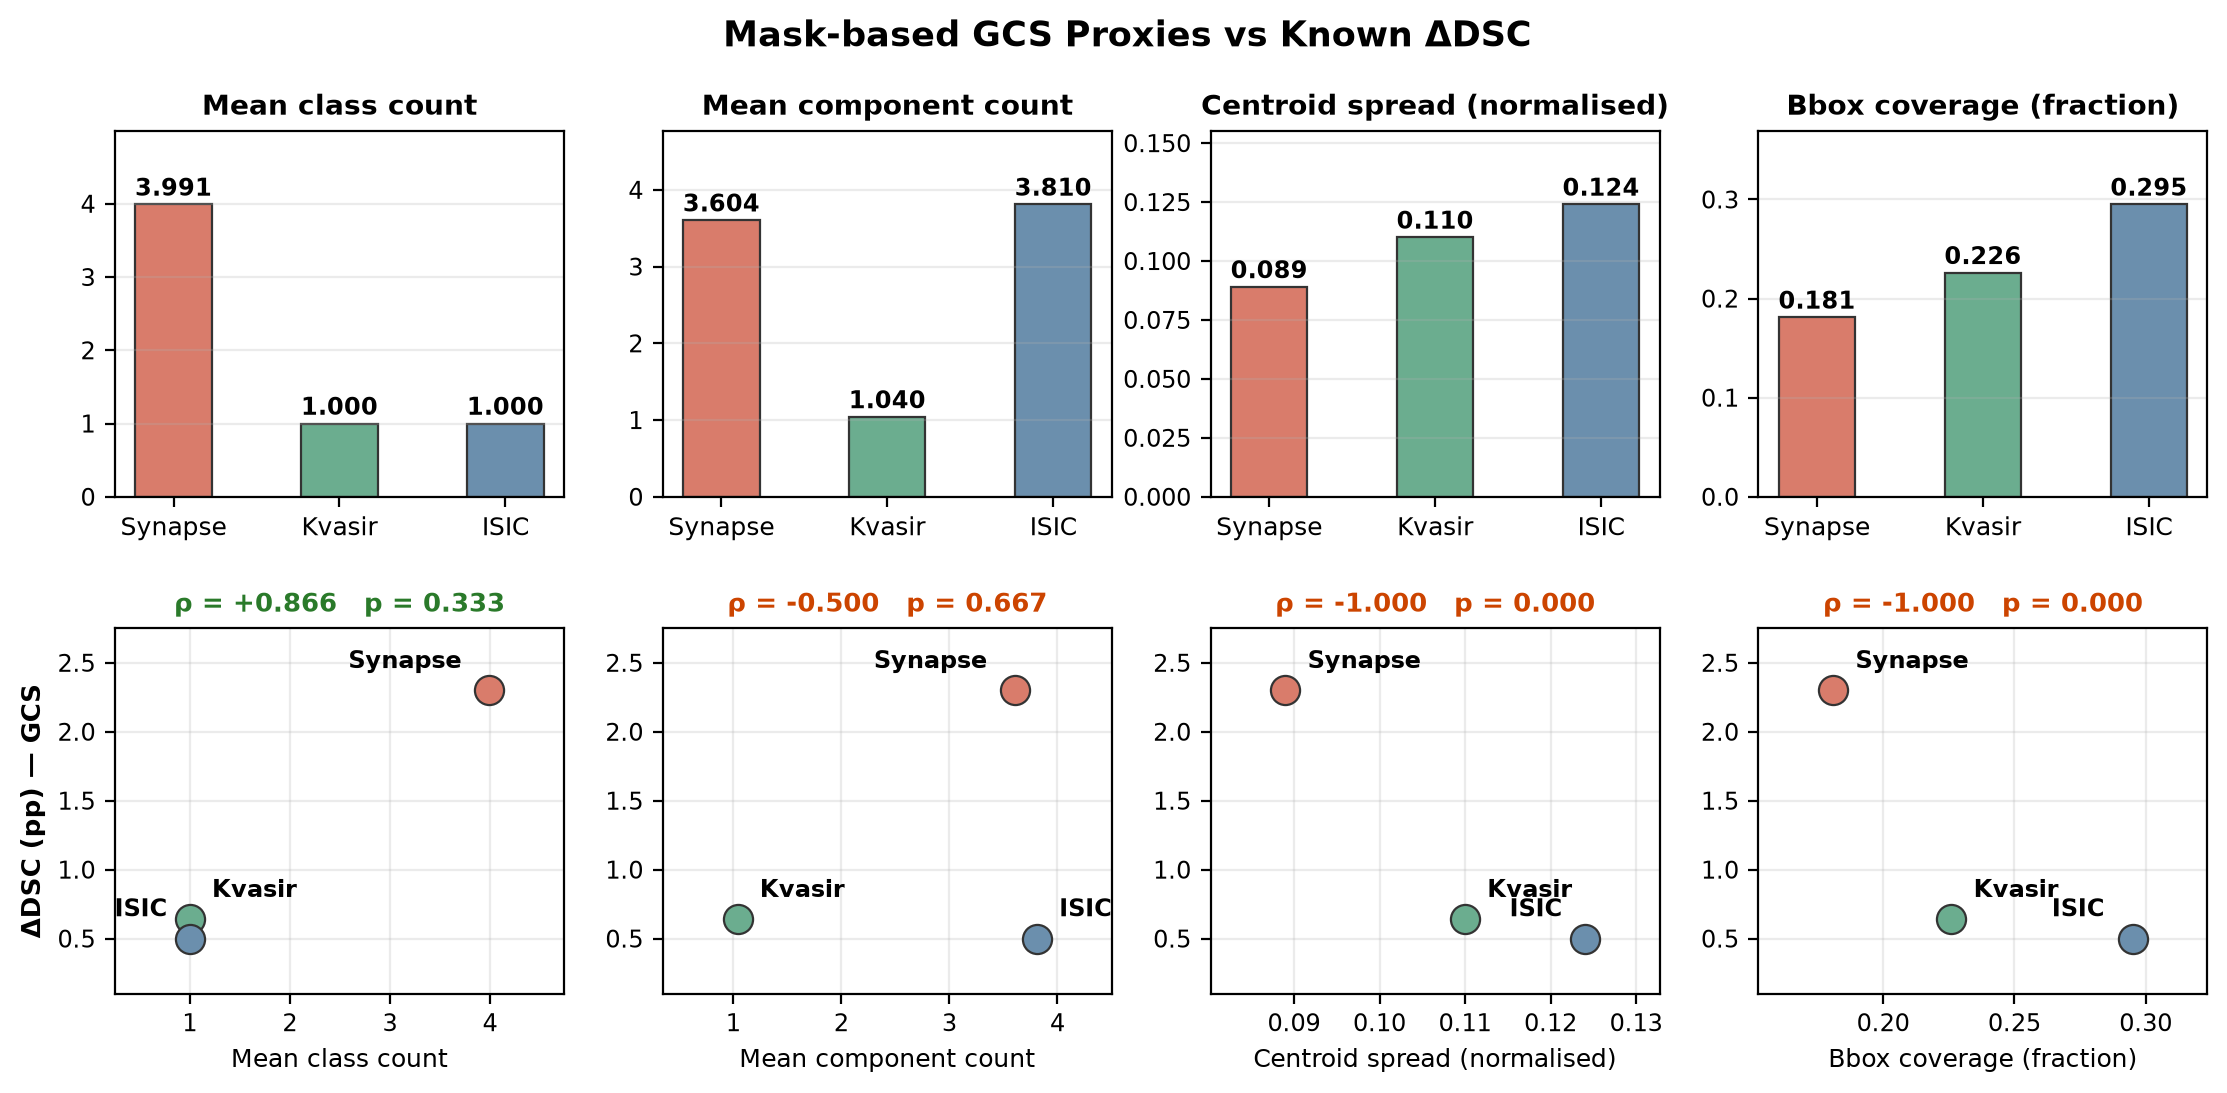
\includegraphics[width=\textwidth]{figures/gcs_mask_sanity.png}
  \caption{Mask-based heuristic proxy metrics vs.\ empirical $\Delta$DSC on initial three benchmarks. While class count correlates on 3 datasets ($\rho{=}+0.87$), subsequent causal testing with ACDC (Table~\ref{tab:causal}) disproves class count as a causal mechanism.}
  \label{fig:proxy}
\end{figure*}

\textbf{Elimination rationale:}
\begin{enumerate}
  \item \textbf{SC1 \& SC3 are eliminated:} Synapse exhibits the lowest foreground coverage (7.7\%) and lowest spatial entropy, yet possesses the highest GCS. Large target size or uniform dispersion does not necessitate large attention windows.
  \item \textbf{SC4 is eliminated by saturation:} In pixel space, even single polyps or skin lesions span across multiple $28{\times}28$ windows ($\text{WCR} \approx 1.0$), demonstrating that component-level crossing is ubiquitous and cannot differentiate GCS tiers.
  \item \textbf{SC2 is eliminated on five datasets:} Boundary irregularity correlated with GCS on the initial 3 datasets ($\rho{=}+0.50$) due to CT image sharpness. Adding cardiac MRI (ACDC) and colonoscopy (CVC) drops this correlation to $\rho{=}0.00$, confirming it was a modality confound.
\end{enumerate}

\subsection{Semantic Spatial Dependency (SSD) as the True Mechanism}
\label{sec:ssd}

The sole surviving metric, \textbf{SC5 (Inter-class Window Separation)}, achieves $\rho = +0.89$ across all five datasets. This establishes that GCS is governed by \textbf{Semantic Spatial Dependency (SSD)}: \emph{the degree to which correctly segmenting a target structure requires identifying its spatial relationship relative to other distinct semantic classes}.

\begin{align*}
  \underbrace{\text{Inter-class SSD}}_{\text{Intrinsic task property}}
  &\;\longrightarrow\;
  \underbrace{\text{Cross-structure spatial attention}}_{\text{Representational requirement}} \\
  &\;\longrightarrow\;
  \underbrace{\text{High window sensitivity}}_{\text{Empirical GCS}}.
\end{align*}

\textbf{ACDC as the critical discriminating test.} To verify that SSD, rather than trivial class count ($n_\text{classes}$), governs GCS, the ACDC benchmark serves as a decisive test case. ACDC contains 4 semantic classes (background, RV, Myo, LV). If class count were the cause, ACDC would exhibit high GCS comparable to Synapse. Instead, ACDC exhibits $\Delta\text{DSC} = 0.73$\,pp, clustering tightly with binary tasks (0.50--0.64\,pp).

SC5 explains this precisely: cardiac structures are concentric and co-located within the cardiac silhouette ($\text{SC5} = 0.547$), so local windows capture sufficient multi-class context. In contrast, Synapse organs are dispersed across the entire abdominal cavity ($\text{SC5} = 0.9996$), where windowed attention at $M{=}7$ cannot attend to neighboring reference organs. Near-complete inter-class spatial separation is the prerequisite for high GCS.

\begin{table}[tb]
  \caption{Per-organ DSC (\%) and window sensitivity ($\Delta$DSC) on Synapse (gate=pam, $r{=}32$, $n{=}4$ window sizes). Sorted by $\Delta$DSC descending.}
  \label{tab:per_organ}
  \centering
  \setlength{\tabcolsep}{3.5pt}
  \small
  \begin{tabular}{lccccr}
    \toprule
    Organ & $M{=}7$ & $M{=}28$ & $M{=}56$ & $M{=}112$ & $\Delta$DSC \\
    \midrule
    Gallbladder & 65.2 & 68.6 & 62.2 & 64.9 & \textbf{6.45\,pp} \\
    Stomach     & 73.8 & 78.7 & 75.5 & 77.0 & \textbf{4.97\,pp} \\
    Kidney (R)  & 78.1 & 82.2 & 82.1 & 80.5 & \textbf{4.16\,pp} \\
    Spleen      & 87.5 & 89.4 & 85.9 & 86.4 & 3.52\,pp \\
    Pancreas    & 60.6 & 62.7 & 61.6 & 62.7 & 2.05\,pp$^\dagger$ \\
    Kidney (L)  & 82.5 & 84.5 & 84.4 & 82.5 & 2.02\,pp \\
    Aorta       & 87.6 & 88.0 & 86.1 & 87.8 & 1.89\,pp \\
    Liver       & 93.7 & 93.3 & 93.4 & 93.6 & \textbf{0.39\,pp} \\
    \midrule
    Mean        & 78.6 & 80.9 & 78.9 & 79.4 & 2.30\,pp \\
    \bottomrule
  \end{tabular}
  \par\vspace{5pt}
  \parbox{\columnwidth}{\footnotesize $^\dagger$Pancreas scores 60--63\% across all windows, reflecting a general segmentation ceiling rather than low SSD.}
\end{table}

\textbf{Within-dataset organ-level validation.} As shown in Table~\ref{tab:per_organ}, organ sensitivities within Synapse directly mirror their anatomical SSD:
\begin{itemize}
  \item \textbf{High-SSD structures:} The gallbladder ($\Delta\text{DSC} = 6.45$\,pp) is small and variable, located at the liver fossa; its identification relies entirely on global liver-gallbladder context. The stomach ($\Delta\text{DSC} = 4.97$\,pp) varies drastically in fill state, requiring adjacent organ boundaries for localization.
  \item \textbf{Low-SSD structures:} The liver ($\Delta\text{DSC} = 0.39$\,pp) is the dominant anatomical landmark recognizable from local parenchymal texture alone. The aorta ($\Delta\text{DSC} = 1.89$\,pp) follows a rigid vertical cylindrical trajectory, rendering it largely window-robust.
\end{itemize}

\subsection{Spatial Attention Allocation and Locality Prior}
\label{sec:attn_allocation}

Why does windowed attention actively outperform global attention on low-SSD tasks? Figure~\ref{fig:attn_map} visualizes the spatial attention distribution ($\|\text{output} - \text{input}\|_2$) for windowed ($M{=}7$) vs.\ global ($M{=}112$) PAM on Kvasir-SEG polyp images.

\begin{figure}[ht]
  \centering
  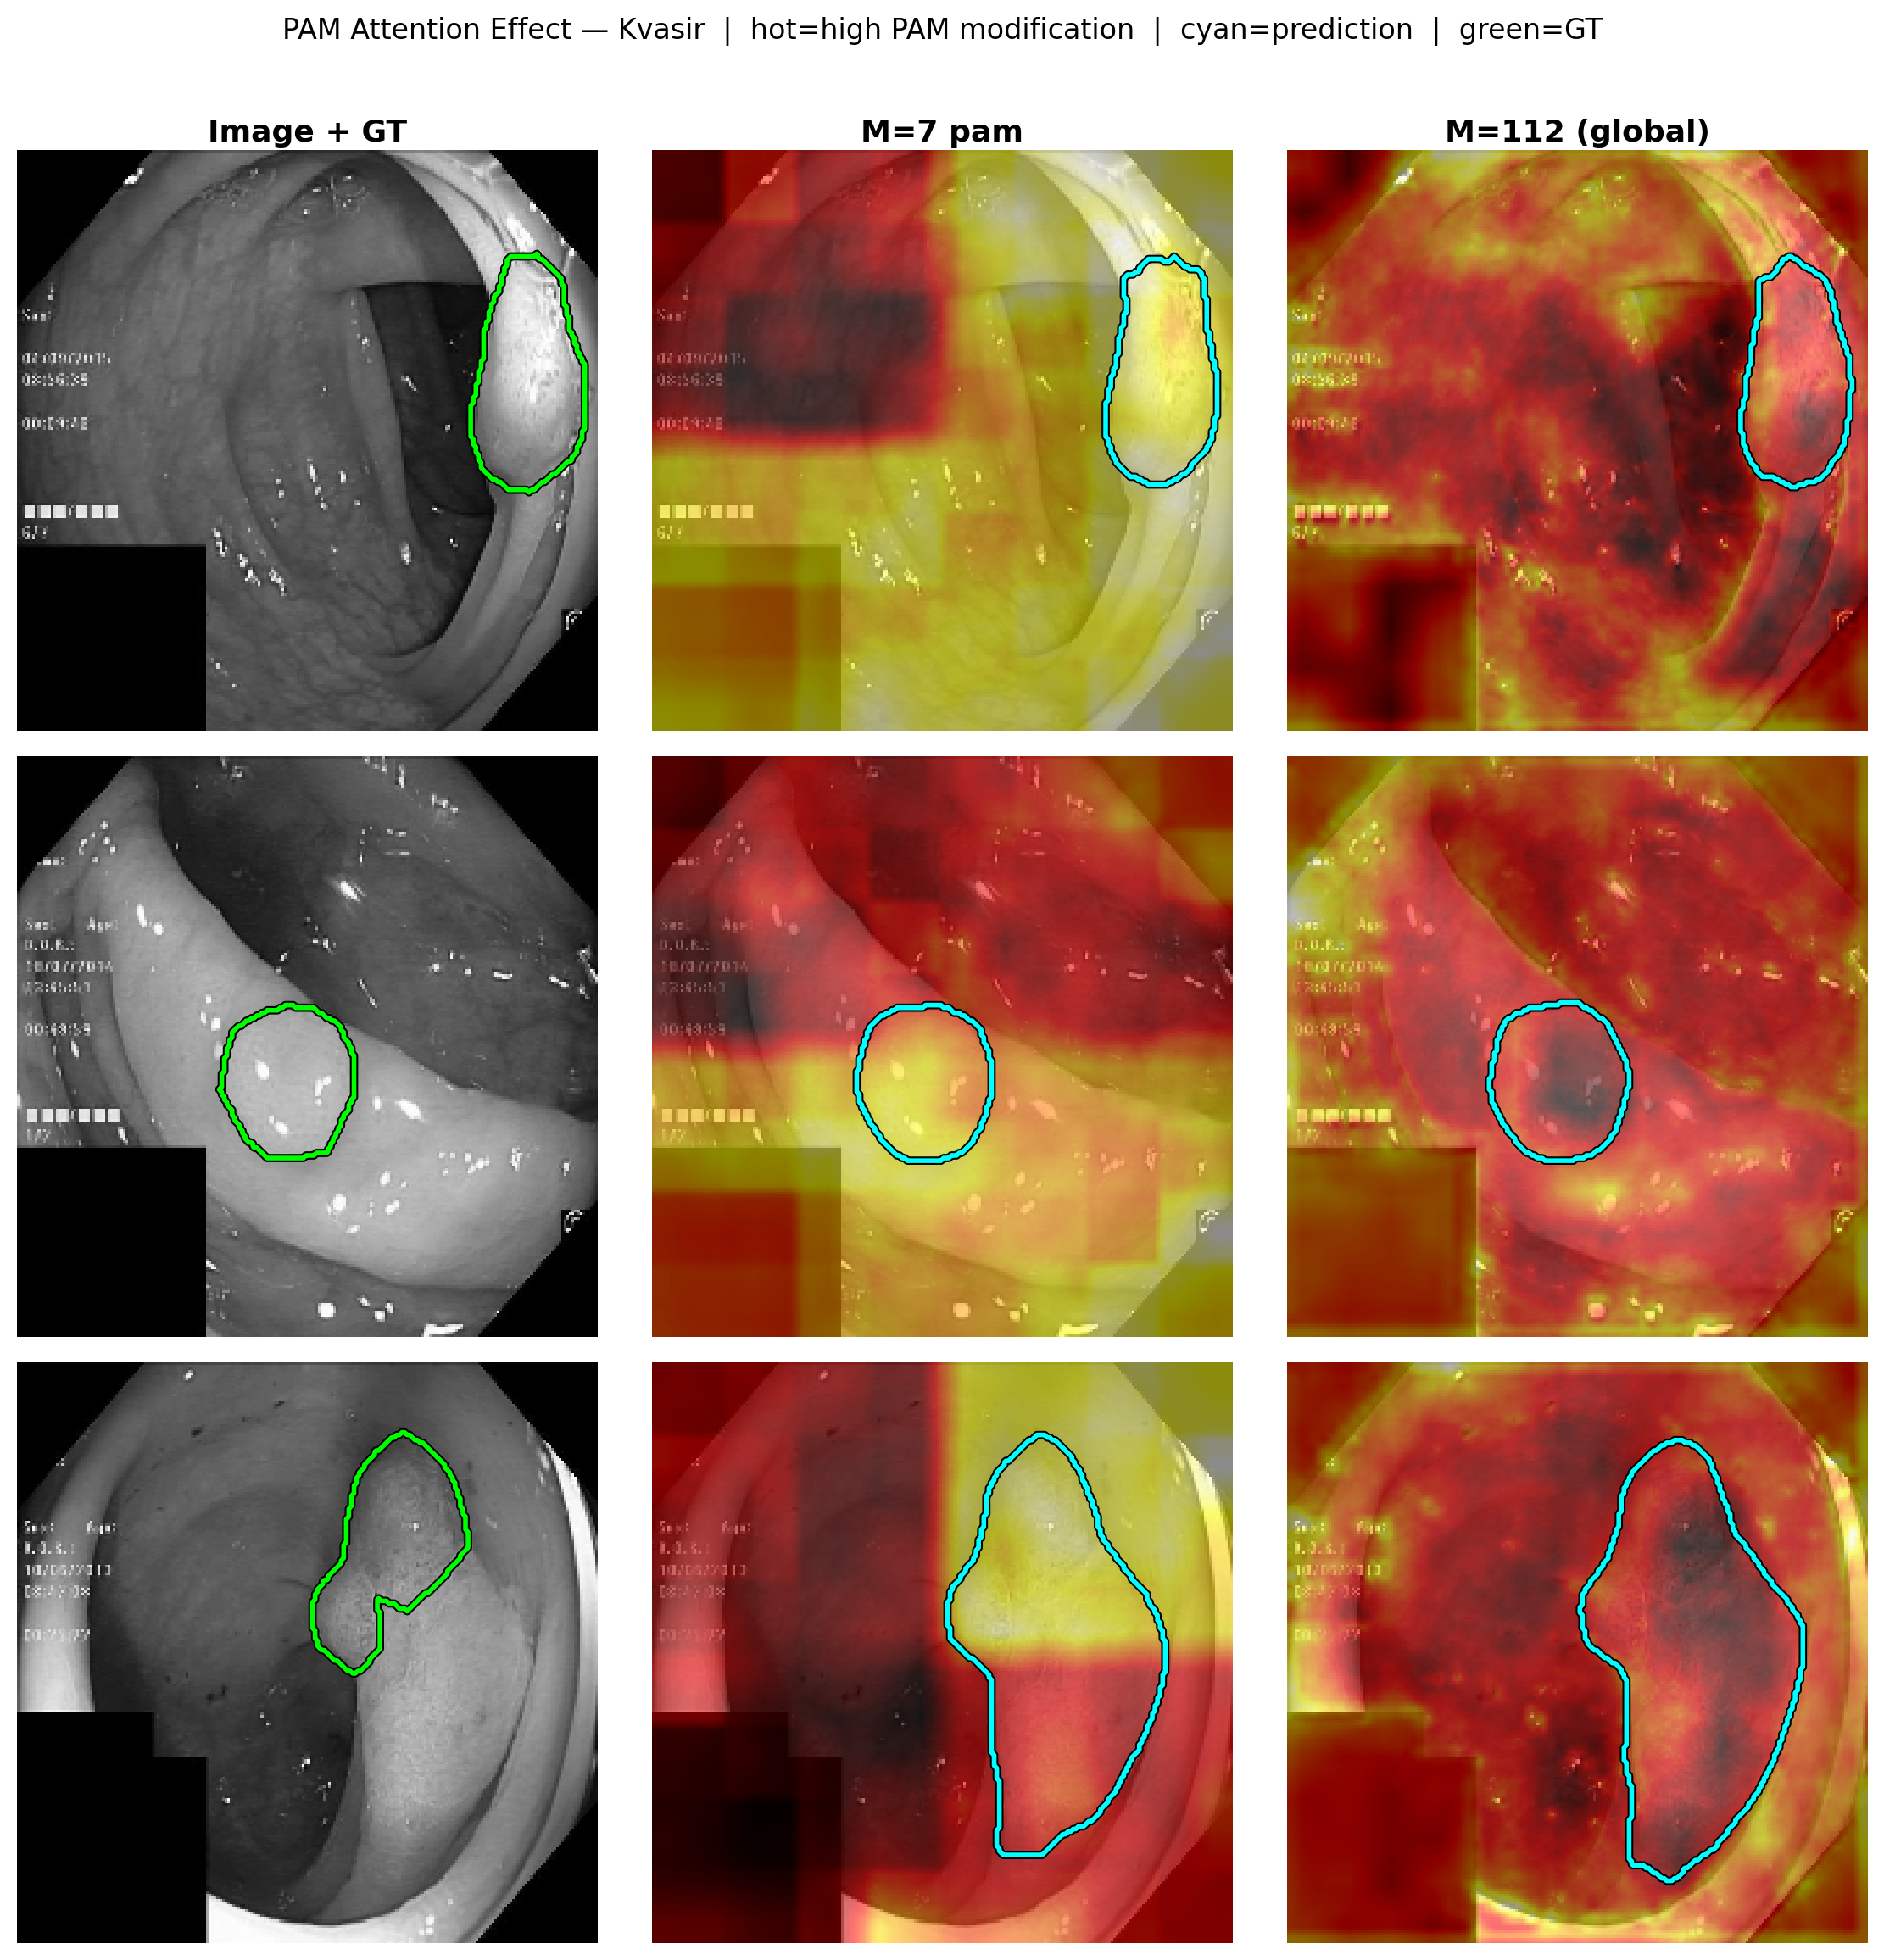
\includegraphics[width=\columnwidth]{figures/attn_Kvasir_M7_r32_pam_vs_M112.png}\\[-4pt]
  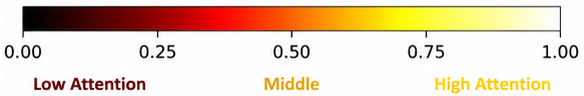
\includegraphics[width=0.68\columnwidth]{figures/hot_color_code.png}
  \caption{PAM contribution maps ($\|\text{output} - \text{input}\|_2$, normalized per-panel) on Kvasir-SEG polyp images. Windowed attention ($M{=}7$) concentrates on polyp boundaries, whereas global attention ($M{=}112$) disperses into surrounding tissue.}
  \label{fig:attn_map}
\end{figure}

Quantitative measurement across 10 test samples confirms that windowed attention concentrates \textbf{62.3\%} of its energy on the polyp region, compared to only \textbf{34.2\%} for global attention ($1.82\times$ concentration ratio, consistent across 9/10 cases). In low-SSD tasks, global attention disperses representational capacity into irrelevant background parenchyma; constraining attention to local windows acts as an inductive bias that sharpens boundary delineation and filters spurious distant interactions.
